% Coordinatewise order leaves pairs incomparable. Lexicographic order is a single chain.
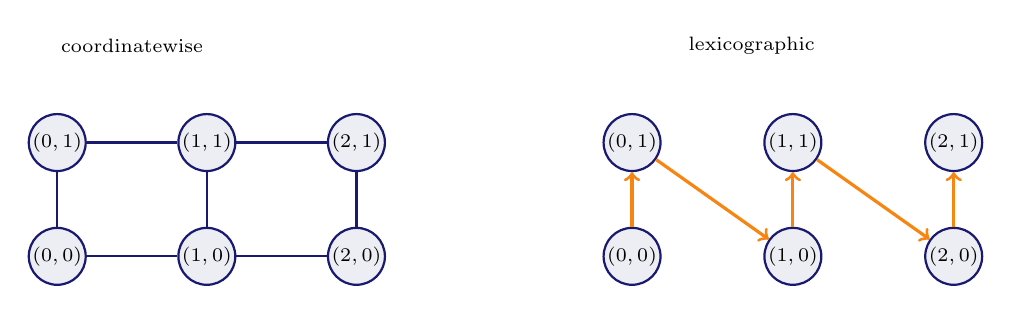
\begin{tikzpicture}[x=0.95cm,y=0.85cm,
  p/.style={circle,draw=MidnightBlue,thick,fill=MidnightBlue!8,inner sep=0.5pt,minimum size=7.2mm,font=\scriptsize}]
  % coordinatewise
  \node[font=\scriptsize] at (1,3.15) {coordinatewise};
  \node[p] (a00) at (0,0) {$(0,0)$};
  \node[p] (a10) at (2,0) {$(1,0)$};
  \node[p] (a20) at (4,0) {$(2,0)$};
  \node[p] (a01) at (0,1.7) {$(0,1)$};
  \node[p] (a11) at (2,1.7) {$(1,1)$};
  \node[p] (a21) at (4,1.7) {$(2,1)$};
  \draw[MidnightBlue,thick] (a00)--(a10)--(a20);
  \draw[MidnightBlue,thick] (a01)--(a11)--(a21);
  \draw[MidnightBlue,thick] (a00)--(a01);
  \draw[MidnightBlue,thick] (a10)--(a11);
  \draw[MidnightBlue,thick] (a20)--(a21);
  % lex
  \begin{scope}[xshift=7.3cm]
    \node[font=\scriptsize] at (1.6,3.15) {lexicographic};
    \node[p] (b00) at (0,0) {$(0,0)$};
    \node[p] (b01) at (0,1.7) {$(0,1)$};
    \node[p] (b10) at (2.15,0) {$(1,0)$};
    \node[p] (b11) at (2.15,1.7) {$(1,1)$};
    \node[p] (b20) at (4.3,0) {$(2,0)$};
    \node[p] (b21) at (4.3,1.7) {$(2,1)$};
    \draw[BurntOrange,line width=1.15pt,->] (b00) -- (b01);
    \draw[BurntOrange,line width=1.15pt,->] (b01) -- (b10);
    \draw[BurntOrange,line width=1.15pt,->] (b10) -- (b11);
    \draw[BurntOrange,line width=1.15pt,->] (b11) -- (b20);
    \draw[BurntOrange,line width=1.15pt,->] (b20) -- (b21);
  \end{scope}
\end{tikzpicture}
